\chapter{Literature Review}
\section{Bearing Capacity}
Foundation\index{Foundataion} is a part of a structure which is meant to transfer load from the superstructure to the ground taking care of shear failure and settlement. In this project we are going to calculate the bearing capacity of soil for the shallow foundation, so only design of shallow foundation is further discussed. Foundations are designed to have an adequate load capacity depending on the type of subsoil/rock supporting the foundation by a geotechnical engineer, and the footing itself may be designed structurally by a structural engineer. The primary design concerns are settlement and bearing capacity. When considering settlement, total settlement and differential settlement is normally considered. Differential settlement is when one part of a foundation settles more than another part. This can cause problems to the structure which the foundation is supporting. Expansive clay soils can also cause problems.

Looking down the pages of the history books, the first ever theory on determination of bearing capacity was given by Rankine\index{Rankine} (1885). He considered the soil mass to be in plastic equilibrium\index{plastic equilibrium} and derived principle stresses\index{principle stress} values for different soil particles to complete his theory. This work was superseded by Prandtl\index{Pradtl} (1920) who considered punching shear failure\index{shear failure!punching} of soil masses to arrive to his formula for determining ultimate bearing capacity. After Prandtl, Hogentogler and Terzaghi\index{Terzaghi} derived another formula for ultimate bearing capacity approximating the actual curved failure surface which had been approximated as logarithmic spiral in theory given by Prandtl\index{Prandtl}.\cite{arora_soil_2004}
\par
Later in 1943, Terzaghi gave a general theory for the bearing capacity under a strip footing making a lot of assumptions like the footing was long enough, shear strength was governed by Mohr-Columb equation\index{mohr columb@Mohr-Columb}, and he also ignored the shear strength of the soil mass that was above the base of the footing.\cite{arora_soil_2004}
\par
Up until now this theory has been revised a lot of times by many famous scientists, so that it can be worked out in various different cases. Meyerhof\index{Meyerhof} (1951), Vesic\index{Vesic} (1973), Skempton\index{Skempton} (1951), Hansen\index{Hansen} (1962), Teng\index{Teng} (1962) etc. have arrived at formulae specific to cases.\cite{arora_soil_2004}
\par

The cases considered in this report assume that the foundation is subjected to centric vertical loading. For the determination of the ultimate bearing capacity of a horizontal footing with a vertical load, the following factors are included: \cite{dunn_fundamentals_1980}
\begin{itemize}
\item The unit weight, shear strength, and deformation characteristics of soil.
\item The size, shape, depth, and roughness of the footing and
\item The water table conditions and initial stresses in the foundation soil.
\end{itemize}

In designing shallow foundations, two possible failure mechanisms\index{failure mechanisms} must be considered. \cite{dunn_fundamentals_1980}
\begin{itemize}
  \item A shear failure\index{shear failure|see{failure mechanisms}} in the soil
  \item Excessive settlement leading to differential settlement\index{diffrential settlement|see{failure mechanisms}} in excess of that tolerable for the supported structures.
\end{itemize}

Bearing capacity is the capacity of soil to support the loads applied to the ground. The bearing capacity of soil is the maximum average contact pressure between the foundation and the soil which should not produce shear failure in the soil. Ultimate bearing capacity is the theoretical maximum pressure which can be supported without failure; allowable bearing capacity is the ultimate bearing capacity divided by a factor of safety. Sometimes, on soft soil sites, large settlements may occur under loaded foundations without actual shear failure occurring; in such cases, the allowable bearing capacity is based on the maximum allowable settlement. Some terms used in bearing capacity are:
\begin{itemize}
\item \textbf{Ultimate bearing capacity($q_u$):} The ultimate bearing capacity is the gross pressure at the base of foundation at which soil fails in shear.

\item \textbf{Net ultimate bearing capacity($q_{nu}$):} It is the ultimate pressure per unit area of the foundation that can be supported by the soil in excess of the pressure caused bt the surrounding soil at the foundation level. It is given as
\begin{equation}
q_{nu} = q_u – q
\end{equation}
where, $q_u$ = ultimate bearing capacity (gross), $q$ = surcharge

\item \textbf{Net Safe Bearing Capacity($q_{ns}$):} It is net pressure that can be applied to soil considering only shear failure. It can be obtained by
\begin{equation}
q_{ns} = \frac{q_u}{FOS}
\end{equation}
where, FOS = factor of safety, which is usually taken as 3.0

\item \textbf{Gross Safe Bearing Capacity($q_{s}$):} It is maximum gross pressure which the soil can carry safetly without shear failure. It is equal to net safe bearing capacity plus the original overburden pressure. ie.
\begin{equation}
q_s = q_{ns} + q
\end{equation}

\item \textbf{Net Safe Settlement Pressure($q_{n\rho}$):} It is net pressure which soil can carry without excessive settlement. For individual footing it is taken between 25mm and 40mm.

\item \textbf{Net Allowable Bearing Pressure($q_{n\rho}$):} It is net bearing bearing pressure which can be used for the design of foundation. As there should be no shearing failure and settlement should also be within the limits, this is smaller of the $q_{ns}$ and $q_{n\rho}$. It is given as
\begin{equation}
q_{na} = \begin{cases}
    q_{ns}, & \text{if } q_{n\rho} > q_{ns}\\
	q_{n\rho}, & \text{if } q_{ns} > q_{n\rho}
	\end{cases}
\end{equation}
\end{itemize}

\subsection{Requirement for design and construction of foundation}
The design and the construction of a well-performing foundation must possess some basic requirements: 
\begin{itemize}
	\item 	The design and the construction of the foundation are done such that it can sustain as well as transmit the dead and the imposed loads to the soil. This transfer has to be carried out without resulting in any form of settlement that can result in any form of stability issues for the structure.
	\item Differential settlements can be avoided by having a rigid base for the foundation. These issues are more pronounced in areas where the superimposed loads are not uniform in nature.
	\item Based on the soil and area it is recommended to have a deeper foundation so that it can guard any form of damage or distress. These are mainly caused due to the problem of shrinkage and swelling because of temperature changes.
	\item The location of the foundation chosen must be an area that is not affected or influenced by future works or factors.
\end{itemize}

\subsection{Types of foundation}
The two types of foundation are:-
\begin{itemize}
  \item Shallow Foundation\index{Foundation!Shallow}
  \par
  Shallow foundations, often called footings, are usually embedded about a metre or so into soil. One common type is the spread footing which consists of strips or pads of concrete (or other materials) which extend below the frost line and transfer the weight from walls and columns to the soil or bedrock.
  \item Deep Foundation
  \par
  A deep foundation is used to transfer the load of a structure down through the upper weak layer of topsoil to the stronger layer of subsoil below.
\end{itemize}

\subsection{Choice for type of foundation}
The choice of the appropriate type of foundation is governed by some important factors such as
\begin{itemize}
	\item The nature of the structure.
	\item The load exerted by the structure.
	\item The subsoil characteristics.
	\item The allotted cost of foundations.
\end{itemize}

\subsection{Three modes of shear failure}
\subsubsection{General Shear Failure}
A continuous failure surface is developed between the edges of the footing which extends up to the ground. As the applied pressure through the footing increases to the range of ultimate bearing capacity, plastic conditions develop around the edge of the footing that spread downward and then outward to the ground surface. Equilibrium is developed along that failure surface. Heave is seen on both sides of the footing. This mode of failure prevails in very dense soil.
\subsubsection{Local shear failure}
This mode of failure prevails in highly compressible soil and the failure mode is characterized by occurrence of relatively large settlement. Partial development of the state of plastic equilibrium occurs and the failure surface does not extend to the ground surface. Slight heave formation occurs on the surface.
\subsubsection{Punching Shear Failure}
It occurs when there is relatively high compression of soil under footing accompanied by shearing in the vertical direction around the edges of the footing. Failure is not accompanied by any heaving or any tilting. This mode of failure prevails in a soil of low compressibility and where the foundation is located at a significant depth.


\subsection{Factors affecting FOS}
Important Features Affecting Factor of Safety
\begin{itemize}
\item	Type of structure permanent or temporary.
\item	Sensitivity of structure.
\item	Extent of soil exploration.
\item	Nature of loading considered and assumption made in the design.
\item	Extent of quality control during construction.
\end{itemize}
It is recommended that the factor of safety should be between 2 and 4. These values are given in Table ~\ref{fs-table}.

\begin{table}
\caption{Recommended factor of safety}
\label{fs-table}
\begin{tabularx}{\textwidth}{ |X|X|X|X| }
\hline
\multirow{2}{*}{Typical Structure} & \multirow{2}{*}{\shortstack[l]{Characteristics of\\ the category}} & \multicolumn{2}{ c |}{Soil Exploration} \\
\cline{3-4}
 & & Through & Limited \\
\hline
 Railway bridge, Warehouses, blast furnaces, silos, hydraulic retaining walls & Maximum design load likely to occur often, consequence of failure disastrous & 3.0 & 4.0 \\
\hline
 Highway bridge, light industrial and public buildings & Maximum design load may occur occasionally, consequence of failure serious & 2.5 & 3.5 \\
\hline
 Apartments and office buildings & Maximum design load unlikely to occur & 2.0 & 3.0 \\
\hline
\end{tabularx}
\end{table}

\subsection{Factors affecting Bearing Capacity of Soil}
Factors affecting the Bearing Capacity of the soil are:\\
\begin{minipage}[t]{0.4\linewidth}
\begin{itemize}
\item	Type of soil.
\item	Unit weight of soil.
\item	Surcharge load.
\item	Depth of foundation.
\item	Mode of failure.
\end{itemize}
\end{minipage}\ignorespaces%\hspace{1.5cm}
\begin{minipage}[t]{0.5\linewidth}
\begin{itemize}
\item	Shape and size of footing.
\item	Depth of water table.
\item	Eccentricity in footing load.
\item	Inclination of ground.
\item	Inclination of base of foundation.
\end{itemize}
\end{minipage}\\

\subsection{Site Investigation Requirements}
Site exploration\index{site exploration} shall be carried out by digging test pits, two as a minimum, and more if the subsurface soil condition shows a significant variation in soil type. Generally, the minimum depth of exploration for a building covered by this MRT shall be 2 m. In hilly areas, exploration up to the depth of sound bed-rock, if it lies shallower than 2 m, should suffice. No exploration shall be required if the site is located on rock or on fluvial terraces (Tar) with boulder beds. The soil encountered in the test pits should be classified as per Table ~\ref{foundation-soil-classification}.
\begin{table}
  \centering
  \caption{Foundation Soil Classification and Safe bearing Capacity}
  \label{foundation-soil-classification}
  \begin{tabular}{|p{0.5\linewidth}|p{0.17\linewidth}|p{0.25\linewidth}|}
  \hline \bfseries{Type of foundation material} & \bfseries{Foundation Classification} & \bfseries{Presumed Safe Bearing Capacity($kN/m^2$)}\\
  \hline Rocks in different state of weathering, boulder bed, gravel, sandy gravel and sand gravel mixture, dense or loose coarse to Medium sand offering high resistance to penetration with excavated by tools, stiff to medium clay which is readily indented with a thumb nail. & Hard & \verb">" 200\\
  \hline Fine sand and silt (dry lumps easily pulverized by the finger), moist clay and sand clay mixture which can be indented with strong thumb pressure & Medium & \verb">" 150 and \verb"<" 200\\
  \hline Fine sand, loose and dry; soft clay indented with moderate thumb pressure & Soft & \verb">" 100 and \verb"<" 150\\
  \hline
  \end{tabular}
\end{table} 
\subsection{Standard Penetration Test}
The SPT\index{SPT} is an in-situ dynamic penetration test designed to provide information of the geotechnical engineering properties of soils. The test is conducted in a bore hole\index{bore hole} by means of a standard split spoon sampler. Once the drilling is done to the desired depth, the drilling tool is removed and the sampler is placed inside the bore hole. By means of a drop hammer\index{drop hammer} of 63.5kg mass falling through a height of 750mm at the rate of 30 blows per minute, the sampler is driven into the soil. This is as per IS -2131:1963.The number of blows of hammer required to drive a depth of 150mm is counted. Further it is driven by 150 mm and the blows are counted. Similarly, the sampler\index{sampler} is once again further driven by 150mm and the number of blows recorded. The number of blows recorded for the first 150mm not taken into consideration. The number of blows recorded for last two 150mm intervals are added to give the standard penetration number\index{SPT!N} (N) in other words no of blows required for 150mm penetration beyond seating drive of 150mm. If the number of blows for 150mm drive exceeds 50, it is taken as refusal and the test is discontinued. The standard penetration number is corrected for dilatancy correction\index{correction!dilatancy} and overburden correction\index{correction!overburden}. There are many parameters of soils which can be correlated with SPT N-value, such as density, undrained shear strength, friction angle, modulus, etc. SPT N-value is accepted as an important indicator and is most widely used to describe soil characteristics\index{soil characterstics}.\cite{mahoto_bearing_2012}
\subsubsection{Problems with SPT}
The Standard Penetration Test recovers a highly disturbed sample, which is generally not suitable for tests which measure properties of the in-situ soil structure, such as density, strength, and consolidation characteristics. However, this results in blow counts which are not easily converted to SPT N-values.  Many conversions have been proposed, some of which depend on the type of soil sampled, making reliance on blow counts with non-standard samplers problematic.
\par
Standard Penetration Test blow counts do not represent a simple physical property of the soil, and thus must be correlated to soil properties of interest, such as strength or density.
\subsubsection{SPT Correction for field procedure}
Dilatancy correction is done for fine sand /silt and below water table and N $>$ 15.
\begin{equation}
N'= 15 + \frac{1}{2} (N - 15)
\end{equation}

The SPT values have been corrected in accordance with the proposal of Skempton\index{Skempton}, (1986) and Liao and Whitman (1987) as outlined below with consideration of field procedure, hammer efficiency, borehole diameter, and sample and rod length. Correction of SPT N-value\index{SPT!correction} using the relation after Skempton (1986) \cite{panthi_bearing_2018}
\begin{equation}
N_{60cs}= E_m * C_B * C_s * C_R * \frac{N'}{0.6}
\end{equation}\\
\begin{minipage}[t]{0.48\linewidth}
\vspace{0pt}
  where,\\
  $E_m$ = 0.55 for hand drop hammer\\
  $C_B$ = 1 for 65-115mm diameter\\
  $C_S$ = 1.0 for standard sampler\\
\end{minipage}
\hfill
\begin{minipage}[t]{0.48\linewidth}
\vspace{0pt}
,\begin{math}
  C_R = \begin{cases}
    0.70, & \text{for length 0-2.99m} \\
    0.75, & \text{for length 3-3.99m} \\
    0.85, & \text{for length 4-5.99m} \\
	0.95, & \text{for length 6-9.99m} \\
    1.00, & \text{for length $>$ 10m}
    \end{cases}
\end{math}
\end{minipage}

The overburden correction is done as
\begin{gather}
C_\sigma = 9.78 \sqrt{ \frac{1}{\sigma_v'} } \le 1.7 \\ 
N_{60} = N_{60cs} * C_\sigma
\end{gather}

\subsection{Some Empirical Relationships} \label{emp-form}
Peak\index{Peak}, Hansen\index{Hansen} \& Thompson\index{Thompson} (1974)\cite{kulhawy_manual_1990}
\begin{gather}
{\phi}_{deg}=27.1+0.3*N_{60}-0.00054*N_{60}^2 \label{phi-form}\\
{\gamma}_{sat}(kN/m^3)= \begin{cases}
    16.8+0.15*N_{60}, & \text{for cohesive soil}\\
    16+0.1*N_{60}, & \text{for cohesion less soil}
    \end{cases}\\
\frac{C_u}{P_a} = 0.29*N_{60}^{0.72} \label{cu-form}
\end{gather}
where, $P_a$ = 100 $kN/m^2$

\subsection{Relation to packing ratio}
Table ~\ref{cbsf-table} show relation of SPT-N\index{SPT!N} to packing ratio.

\begin{table}
  \centering
  \caption{Correlation between SPT-N value and soil packing(Meyerhof 1956)}
  \label{cbsf-table}
  \begin{tabular}{|c|c|l|}
  \hline &\bfseries{SPT N3(1ft)} & \bfseries{Soil packing} \\
  \hline \multirow{5}{*}{\begin{sideways}\bfseries{Cohesionless}\end{sideways}} & \verb"<" 4 & Very loose \\
  \cline{2-3} & 4-10 & Loose \\
  \cline{2-3} & 10-30 & Compact \\
  \cline{2-3} & 30-50 & Dense \\
  \cline{2-3} & \verb">" 50 & Very Dense \\
  \hline \multirow{5}{*}{\begin{sideways}\bfseries{Cohesive}\end{sideways}} & \verb"<" 2 & Very soft \\
  \cline{2-3} & 2-4 & Soft \\
  \cline{2-3} & 4-8 & Firm \\
  \cline{2-3} & 8-15 & Stiff \\
  \cline{2-3} & 15-30 & Very Stiff \\
  \cline{2-3} & \verb">" 30 & Hard \\
  \hline 
  \end{tabular}
\end{table}

\subsection{Terzaghi’s Bearing Capacity Theory}
Based on Terzaghi’s bearing capacity theory, column load P is resisted by shear stresses at edges of three zones under the footing and the overburden pressure, q ($=\gamma D$) above the footing.  The first term in the equation is related to cohesion of the soil. The second term is related to the depth of the footing and overburden pressure. The third term is related to the width of the footing and the length of shear stress area. The bearing capacity factors, Nc, Nq, Ng, are function of internal friction angle, $\phi$.
The general bearing capacity derived by Terzaghi\index{Terzaghi} for square footing are
\begin{gather}
Q_u = 1.3 * C * N_c + q_0 * N_q * R_{W1} + 0.4 * {\gamma} * B * N_{\gamma} * R_{W2} \\
N_c = \cot \phi (N_q - 1)\\
N_q = \exp ^ 2 (\frac{3\phi}{4} - \frac{\phi}{2}) \frac{\tan \phi}{2 \cos ^2 (45 + \frac{\phi}{2})}\\
N_{\gamma} = \frac{\tan \phi (\frac{K_p}{\cos ^2 \phi} - 1)}{2}\\
K_p= \tan ^ 2 (45 + \frac{\phi}{2})\\
R_{W1} = 0.5 (1 +\frac{D_{W1}}{D_f}) \text{, if } (\frac{D_{W1}}{D_f})\le 1 \\
R_{W2} = 0.5 (1 +\frac{D_{W2}}{B})\text{, if } (\frac{D_{W2}}{B})\le 1
\end{gather}

Assumptions in Terzaghi’s Bearing Capacity Theory.
\begin{enumerate}
\item Depth of foundation is less than or equal to its width.
\item Base of the footing is rough.
\item Soil above bottom of foundation has no shear strength; it is only a surcharge load against the overturning load.
\item Surcharge upto the base of footing is considered.
\item Load applied is vertical and non\-eccentric.
\item The soil is homogenous and isotropic.
\item L/B ratio is infinite.
\end{enumerate}

\subsection{Meyerhof’s Bearing Capacity Theory}
In 1951, Meyerhof\index{Meyerhof} published a bearing capacity theory which could be applied to rough shallow and deep foundations. Meyerhof (1951, 1963) proposed a bearing-capacity equation similar to that of Terzaghi but included a shape factor $S_q$ with the depth term $N_q$. He also included depth factors and inclination factors.\cite{mey_book}
\par
The failure surface at ultimate load under a continuous foundation as assumed by Meyerhof (1951) is shown in Figure ~\ref{meyerhof-analysis}. In this figure, abc is the elastic triangular wedge shown in Figure ~\ref{meyerhof-analysis}, bcd is the radial shear zone with cd being an arc of a log spiral, and bdef is a mixed shear zone in which the shear varies between the limits of radial and plane shear depending on the depth and roughness of the foundation. The plane be is referred to as an equivalent free surface. The normal and shear stresses on the plane be are $P_o$ and $s_o$, respectively. The superposition method is used to determine the contribution of cohesion (c), on the ultimate bearing capacity $Q_u$ of the continuous foundation and can be expressed as
\begin{gather}
Q_u = C * N_c * S_c * d_c + q_0 * N_q * S_q * d_q + 0.5 * {\gamma} * B * N_{\gamma}*S_{\gamma}*d_{\gamma}\\
N_c = \exp^{\pi * \tan(\phi)} * \tan^2 ( 45 + \frac{\phi}{2} )\\
N_q = \cot(\phi)*(N_q - 1)\\
N_{\gamma} = (N_q-1) * \tan(1.4*\phi)\\
S_c = 1 + 0.2 * K_p\\
S_q=1+0.1*K_p\\
S_{\gamma}=1+0.1*K_p\\
d_c=1+0.2*\sqrt{K_p}*(\frac{D}{B})\\
d_q=d_{\gamma}=1+0.1*\sqrt{K_p}*(\frac{D}{B})\\
K_p= \tan ^ 2 (45 + \frac{\phi}{2})
\end{gather}
\begin{figure}
\centering
\caption{Meyerhof’s Analysis\cite{mey_book}}
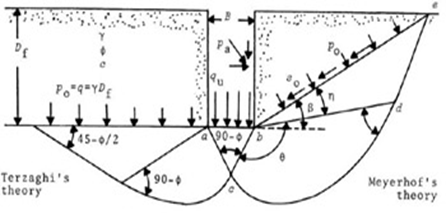
\includegraphics{images/main/meyerhof-analysis.png}
\label{meyerhof-analysis}
\end{figure}

\subsection{Hansen’s Bearing Capacity Theory}
As shown by Milovic (1965), Terzaghi theory gives high ultimate bearing capacity for cohesion less soil which is dangerous and it gives conservative bearing capacity for cohesive soil so Hansen\index{Hansen} (1961) developed equations which are in better agreement with experimental values. Ultimate bearing capacity is given by, \cite{arora_soil_2004}
\begin{gather}
Q_u = C * N_c * S_c * d_c * i_c + q_0 * N_q * S_q * d_q * i_q + 0.5 * {\gamma} * B * N_{\gamma}*S_{\gamma}*d_{\gamma} * i_{\gamma}\\
N_c = \exp^{\pi * \tan(\phi)} * \tan^2 ( 45 + \frac{\phi}{2} )\\
N_q = \cot(\phi)*(N_q - 1)\\
N_{\gamma} = 1.8 * (N_q-1) * \tan(\phi)
\end{gather}
For square footing,
$S_c = S_q = S_{\gamma} = 1.3$
\begin{gather}
d_c=d_q = 1+0.35*(\frac{D}{B})\\
d_{\gamma} = 1\\
i_c=1 - \frac{H}{2*c*B*L}\\
i_q=1 - \frac{1.5*H}{V}\\
i_{\gamma} = i_q^2  
\end{gather}

\subsection{Vesic's Bearing Capacity Theory}
Vesic\index{Vesic} (1973) confirmed that the basic nature of failure surfaces in soil as suggested by Terzaghi as incorrect. However, the angle which the inclined surfaces AC and BC make with the horizontal was found to be closer to 45 + $\frac{\phi}{2}$ instead of 45 . The values of the bearing capacity factors , for a given angle of shearing resistance change if above modification is incorporated in the analysis as under: \cite{arora_soil_2004}
\begin{gather}
Q_u = C * N_c * S_c * d_c * i_c + q_0 * N_q * S_q * d_q * i_q + 0.5 * {\gamma} * B * N_{\gamma}*S_{\gamma}*d_{\gamma} * i_{\gamma}\\
N_c = \exp^{\pi * \tan(\phi)} * \tan^2 ( 45 + \frac{\phi}{2} )\\
N_q = \cot(\phi)*(N_q - 1)\\
N_{\gamma} = 2 * (N_q+1) * \tan(\phi)\\
S_c = 1 + \frac{N_q}{N_c}\\
S_q = 1+ \tan(\phi)\\
S_{\gamma} = 0.6, \text{for square footing}\\
d_c=1+0.4*\frac{D}{B}\\
d_q= 1 + 2 * \tan(\phi)*(1-\sin(\phi) )^2*\frac{D}{B}\\
d_{\gamma} = 1 , for \frac{D}{B}<1 , \text{use Hansen value}\\
i_c=i_q = (1-\frac{\alpha}{90})^2\\
i_{\gamma}=(1-\frac{\alpha}{\phi})^2
\end{gather}

\subsection{Teng's method}
Teng expressed the charts given by Terzaghi and Peck (1948) in the form of following formulae. He also added the allowance for increase in preface with depth by introducing a depth factor.
\begin{equation}
q_a = 35 (N-3) (\frac{B+0.3}{B})^2 W_\gamma R_d
\end{equation}
where,
$q_a$ = allowable bearing capacity for 25 mm settlement.,\\
$W_\gamma$ = water table correction factor.\\
$R_d$ = depth factor = $1 + \frac{D_f}{B}$

Also, from shear criteria,
\begin{equation}
q_nu = 0.11 N^2 B {W_\gamma} + 0.33 (100+N^2)D_f*{W_\gamma}
\end{equation}

\subsection{Peck method}
Terzaghi and Peck (1967) gave charts for the safe bearing pressures introducing a total settlement of 25 mm and a differential settlement of 19 mm for different footings. Peck et al (1974) revised the Terzaghi and Peck curves to consider in later research, and gave following equations for the safe settlement pressure.\cite{arora_soil_2004}
\begin{equation}
q_{n\rho} = 0.41 C_w Ns
\end{equation}
Where,
 $q_{n\rho}$ is the safe settlement pressure in $kN/m^2$\\
 $N$ is corrected SPT value\\
 $s$ is settlement in mm\\
 $C_w$ is water table correction factor.
 
We calculate using Peck method bu taking deflection of 25mm so for 25 mm deflection the above equations becomes,
\begin{equation}
q_{n\rho} = 10.25 C_w Ns
\end{equation}
Where water table correction is found using equation,
\begin{equation}
C_w=0.5+0.5 D_w / (D_f + B)
\end{equation}
where,
$D_w$ is Depth of water below ground surface.\\
$D_f$  is depth of footing.\\
$B$ is width of footing.

\subsection{Bowles theory}
The bearing capacity of a soil is given by Terzaghi and Peck was found to be very conservative. Meyerhof (1956,1974) published equation for computing the allowable bearing for a 25 mm settlement, which also underestimated the value. Bowels, for this reason, adjusted the Meyerhof equation by a multiplication factor of 1.5.
\begin{equation}
q_a = \begin{cases}
			\frac{N}{F_1} R_d * W_\gamma, & B \le F_4 \\
			\frac{N}{F_2}(\frac{B+F_3}{B})^2 R_d, & B \textgreater F_4
		\end{cases}
\end{equation}
\begin{equation}
R_d = 1 + 0.33 \frac{D}{B} \le 1.33 
\end{equation} (Meyerhof 1965)
where,\\
$q_a$  = allowable bearing capacity for settlement of 25mm, unit is kPa.,\\
$N$ = For $E_r$ 55\\
$F_1$ = 0.05, $F_2$ = 0.08, $F_3$ = 0.3 ,and $F_4$ = 1.2, for SI units.

\subsection{Finite Element Method}
The finite element method\index{FEM} (FEM) is the most widely used method for solving problems of engineering and mathematical models. Typical problem areas of interest include the traditional fields of structural analysis, heat transfer, fluid flow, mass transport, and electromagnetic potential. The FEM is a particular numerical method for solving partial differential equations in two or three space variables (i.e., some boundary value problems). To solve a problem, the FEM subdivides a large system into smaller, simpler parts that are called finite elements. This is achieved by a particular space discretisation in the space dimensions, which is implemented by the construction of a mesh of the object: the numerical domain for the solution, which has a finite number of points. 
\subsubsection{PLAXIS}
PLAXIS\index{PLAXIS} is a finite element program for geotechnical applications in which soil models are used to simulate the soil behavior. The PLAXIS code and its soil models have been developed with great care. Although a lot of testing and validation have been performed, it cannot be guaranteed that the PLAXIS code is free of errors. Moreover, the simulation of geotechnical problems by means of the finite element method implicitly involves some inevitable numerical and modeling errors. The accuracy at which reality is approximated depends highly on the expertise of the user regarding the modeling of the problem, the understanding of the soil models and their limitations, the selection of model parameters, and the ability to judge the reliability of the computational results. Hence, PLAXIS may only be used by professionals that possess the aforementioned expertise. The user must be aware of his/her responsibility when he/she uses the computational results for geotechnical design purposes.

\subsection{Geographic information system}
Geographical Information System (GIS) is a computer based information system used to digital represent and analyze the geographical features, present on the Earth’s surface and events that taking place on it. The meaning of GIS is to represent digitally is to convert analogue (smooth line) into digital form.
“Every object present on the Earth can be geo-referenced”, is the fundamental key of associating any database to GIS. Here, the term ‘database’ is a collection of information about thing and their relationship to each other and ‘geo referencing’ refers to the location of a layer or coverage in space defined by co-ordinate reference system.

Work on GIS began in late 1950s, but first GIS software came only in late 1970s from lab of the ESRI. Canada was the pioneer in the development of GIS as a result of innovation dating back to early 1960s. Much of the credit for the early development of GIS goes to Roger Tomilson. Evolution of GIS has transformed and revolution and revolutionized and the ways in which planners, engineers, managers etc. conduct the database management and analysis.

GIS is no longer viewed as complicated, expensive tool for geographers and cartographers to plot out maps. It has tremendous potential to affect a wide variety of fields, from community planning and economic development to political district mapping and Engineering solutions. It is used to find location and conditions of that location, trends and patterns of location about the recent changes in location. Also modelling and mapping can be done in GIS.

Map is a small scale representation of Earth’s surface. Representation of earth on a map encounters some distortion in distance, area, shape and direction. It is necessary to apply some kind of scale reduction to represent earth’s features into a map. Well designed map contains title, legend, credits, map scales, mapped area, map symbols, place name and labelling, north arrow, boarder, Inset and graticule.

Every Spatial features needs to be referenced GIS use. Spatial reference systems provide a framework to define positions on the Earth’s surface. We are used to working with coordinate systems, but due to Earth’s irregular system, this method becomes intricate. Here we represent spherical or ellipsoidal surface of earth in flat plane. For that we use projection of earth on a cylindrical surface. This can be done in many methods, we use MUTM (Modified Universal Traverse Mercator) which divides Earth into 120 parts of 3 degree each for using projections, which is slightly better than UTM projection for calculations in Nepal. We use MUTM coordinate system with 84 degree datum.

\subsubsection{QGIS}
QGIS is a free and open-source cross-platform desktop geographic information system (GIS) application that supports viewing, editing, and analysis of geospatial data. It allowing users to analyze and edit spatial information, in addition to composing and exporting graphical maps. It is a good alternative of ArcGIS which is free and has a large community. It is written in C++ available under the conditions of the GPL license. It is based on the C++ crossplattform library Qt from Trolltech. Therefore, it runs on most existing operating systems, including Linux, Unix, Mac OS X and Windows. 

The main focus of QGIS is interactive two dimensional viewing of spatial data. However, there is also functionality for editing vector data and a GRASS plugin to use the analytical functionality of the GRASS program from within the QGIS GUI. QGIS supports a large number of vector and raster formats, including PostGIS, GRASS, Shapefile, GML, WFS, GPX, WMS, GeoTiff, PNG, JPG and many others. QGIS supports reprojecting on-the-fly for vector data.
%--------------------------------------------------------------------------------------------------------------------------------------------------------------
\section{Liquefaction}
\subsection{Introduction}
Liquefaction is one of the major causes of heavy destruction during a seismic event. It occurs in the deposit of loose and saturated sand with certain range of percentage of fines \cite{r11}. The occurrence of liquefaction is distributed around the epicentre and is generally observed near river, lakes owing to the favourable soil properties and the ground water level there.  Loose sand tends to contract during the earthquakes which causes the pore water pressure in the voids to rise, and with the proper drainage not available either due to the deposit being a large one or due to the lower values of permeability of the deposit, which causes the pore water pressure to further rise up to the effective stress, resulting in a temporary loss of shear strength, imparting the liquid like behaviour to the deposit. The liquid like behaviour of the sand deposit introduces large deformations in the structures resting on the ground above the deposit. Lateral spread, sand boiling and surface cracks are the prominent effects observed during a liquefaction event.

Most dramatic illustrations of the damages due to liquefaction to the civil-engineering structures were observed during the 1964 Niigata Earthquake and Alaska Earthquake occurring in the same year. The results of those liquefaction were dramatic bearing failures beneath the buildings, floating of the underground tanks and collapse and damages to several bridges nearer to the epicentre. These events for the first time drew attention of the engineering community towards the scientific study of the phenomenon. Since then, it has frequently been observed, recorded and studied during various major seismic events occurring around the globe. 

The documentation and study of such events have been playing a vital role in prediction of occurrence of liquefaction at a certain place and broadly into the understanding of the phenomenon itself. Several techniques have been developed along the years, which can be broadly be grouped under :
\begin{enumerate}
\item methods that are based off the soil properties which are determined by laboratory testing
\item methods that are based off the In- situ test results
\item methods that are based off numerical modelling
\item combination of laboratory testing and back analysis of any past records of occurrence of liquefaction.
\end{enumerate}

In this report, liquefaction hazard mapping has been done by the 2nd method from site observed SPT values.

The causes of liquefaction during a seismic event can be attributed to the loss of local shear strength due to the undrained conditions being established under the cyclic loading introduced by the shaking. However, the parameters which assist in establishment of such conditions can be separately discussed as follows:

\begin{itemize}
\item Seismic causes
Intensity of the earthquake basically depends upon the magnitude of the earthquake, the distance of the site from the epicentre of the earthquake, the stiffness of the medium the seismic waves travel through and the attenuation of the energy. All these factors dictate the local PGA, which plays essential role for liquefaction to occur.
\item Site Conditions
Liquefaction generally occurs at the places nearer to the water bodies as the land nearby is ever saturated. Moreover, the young deposition of sand with no past history of exposure to the shaking due to the quake with uniform gradation in very loosely packed state makes the site much more vulnerable.
\end{itemize}

The dynamic strength of soil is affected strongly by the characteristics of soil grain such as grain size, grain shape, grain distribution and mineral composition. Seed \cite{r12} presented the relationship between the liquefaction resistance and the mean grain size ($D_{50}$). The liquefaction resistance increases with increasing with the $D_{50}$ of soil specimen. Ishibashi\cite{r14}  showed that for a given mean grain size ($D_{50}$), soil specimen with well-graded grain distribution have lightly greater liquefaction resistance than that with uniform grain size distribution.

Concerning the fine content in a soil, several studies show that the liquefaction resistance of the soil will first go on decreasing with increasing fine content, reach to a minimum value and then go on increasing afterwards. 

Factors affecting the cyclic strength with the level of effect \cite{r13}

\begin{tabularx}{\textwidth}{ |X|X|X| }
\hline
Factors Affecting Liquefaction & Pure Sand & Sand with silt content \\
\hline
Average effective Confining Pressure & R & R \\
\hline
Void Ratio, e & V & V \\
\hline
Saturated degree, Sf & V & V \\
\hline
Over-consolidation Ratio, OCR & L & V\\
\hline
Pre-strain history & V & V\\
\hline
Sample Prepared Method & V & V\\
\hline
Grain Size, Distribution and Mineral Contents & V & V \\
\hline
Frequency of Loading & R & L \\
\hline
Time Effect & R & R \\
\hline
Volume change during shear strain \(\gamma < 0.5 \%\) & U & U \\
\hline
\end{tabularx}

Note:
\begin{tabular}{l l}
V: Major effect factor & L : Minor effect factor\\
R: Light effect factor & U : Significance unknown
\end{tabular}

Regarding the silty soils in specific, so called Chinese Criteria \cite{r20} has been presented in Seed et. Al \cite{r12} , which is as follows:

\begin{itemize}
\item Clay Content (defined as \% finer than 0.005 mm) \textless 15\%
\item Liquid Limit \textless  35
\item Water Content \textgreater 0.9 * Liquid Limit
\end{itemize}

With increasing relative density, it is much unfavourable for the soil element to develop excess pore water pressure. The liquefaction study carried out by Seed \cite{r14} post Nigata earthquake led to the result that the soil liquefaction was much likely to occur when the relative density was about 50\%. Above 70\% silt content hazard of the liquefaction was found substantially low. Mulilis \cite{r15} presented that the liquefaction resistance of soil has liquefaction resistance of soil has linear relationship with the relative density as the relative density of soil is less than 70\%, and the relationship is also a function of confining pressure.

Tokimatsu and Yoshimi \cite{r17} further concluded that the sand with more than 10\% fines have much greater liquefaction resistance than clean sands with same SPT N-values. Liquefaction resistance of soil increases with increasing of the confining stress as demonstrated by Seed \cite{r16}, based on the results of the cyclic triaxial test, however the required cyclic shear stress ratio to develop liquefaction decreases with increasing effective confining pressure.

\subsubsection{Geology of Kathmandu Valley}
Kathmandu valley is geologically characterized by occurrence of fluvio-lacustrine sediments of Pliocene to Quaternary age that comprise Kathmandu complex with Phulchoki and Bhimphedi group as basement rocks. Thickness of sediment deposit is varied according to the location. For instance, the central valley consists unconsolidated sediments of about 550–600 m depth and the depth is limited to 50–70 m at the edges. 

\begin{figure}[!hbt]
\centering
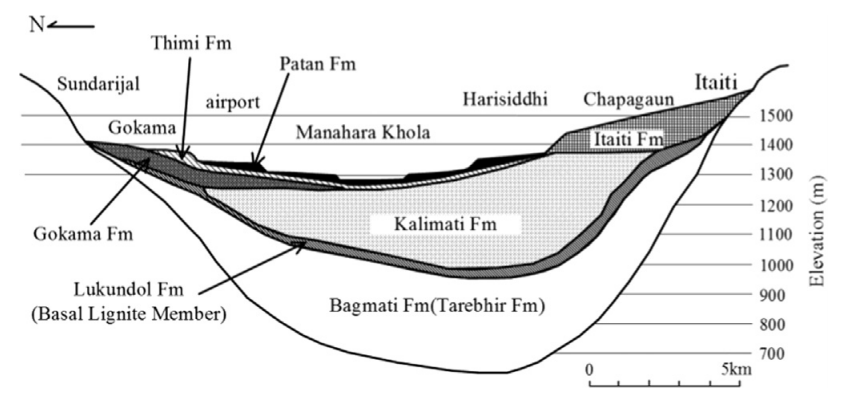
\includegraphics[width=0.75\linewidth,keepaspectratio]{images/main/geological_cross_section.png}
\caption{A schematic cross-section showing the stratigraphic framework and depositional environments of the basin-fill sediments in the Kathmandu Valley (from Sakai \cite{r24}).}
\end{figure}

\subsubsection{Liquefaction Susceptibility Maps of Kathmandu}
UNDP/UNCHS Liquefaction Susceptibility Maps of 1994

The very first attempt to produce liquefaction susceptibility map of Kathmandu valley was done by UNDP/UNCHS in 1994. The analysis was made on the basis of geological and hydrological considerations on the basis of qualitative method developed by Juang\cite{r25}. All Flood plains and some part of central part of valley was presented as the most liquefaction prone area of the whole valley.  As the qualititative method of evaluation of liquefaction potential has it’s own limitations, the study could not produce a comprehensive  map.

\begin{figure}[!hbt]
\centering
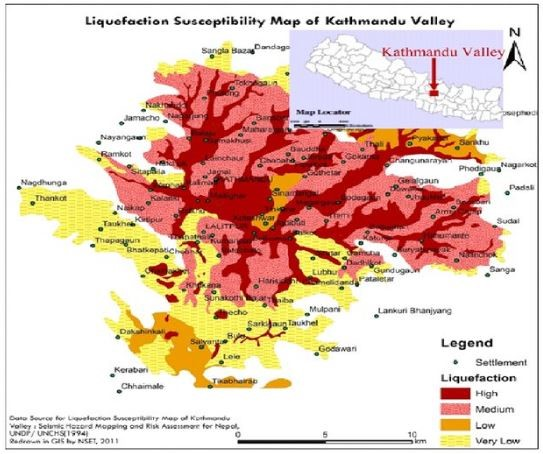
\includegraphics[width=0.75\linewidth,keepaspectratio]{images/main/undp_susceptibility.jpg}
\caption{UNDP/UNCHS Liquefaction Susceptibility Maps of 1994}
\end{figure}

\subsubsection{Map Presented By JICA}

JICA prepared a map in 2002 based on qualitative method of evaluation of Liquefaction Susceptibility, using borehole log data from limited places. The work as carried out under the project “The Project for Assessment of Earthquake Disaster Risk for the Kathmandu Valley in Nepal”. The method proposed by Iwasaki \cite{r26} was used. The map then got revised in 2018 when JICA published a report on seismic risk assessment in Kathmandu Valley. The results of the map were somewhat closed to the results proposed by UNDP back in 1994, considering the aspect of the result that both of the maps showed considerable liquefaction potential in the areas in the flood plains of Bagmati river. The map also showed various places where liquefaction was observed in the recent 2015 Gorkha earthquake and 1934 Bihar Nepal Earthquake.

\begin{figure}[!hbt]
\centering
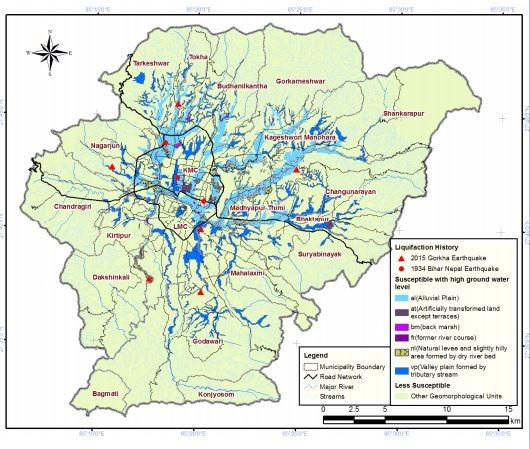
\includegraphics[width=0.75\linewidth,keepaspectratio]{images/main/jica_sus.jpg}
\caption{Liquefaction Susceptibility Map Presented By JICA}
\end{figure}

Liquefaction Susceptibility Map produced by JICA(2018), updated one from that published in 2004.

\subsubsection{Other maps developed throughout the years}

\begin{figure}[!hbt]
\centering
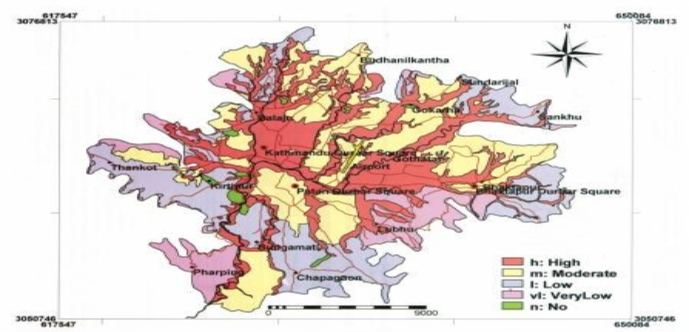
\includegraphics[width=0.75\linewidth,keepaspectratio]{images/main/piya.png}
\caption{ Liquefaction Susceptibility Map (Piya)}
\end{figure}

Piya et al.(2004) have developed one using both of the qualitative and quantitative methods proposed by Juang\cite{r25}, Iwasaki\cite{r26} and Seed and Idriss\cite{r12}. The map divides the valley into 5 categories: no, very low, low, moderate and high on the basis of susceptibility to liquefaction. The core areas of the valley and the areas along the flood plains as indicated previously by other maps were again found to be vulnerable to liquefaction from the study.

Subedi\cite{r28} produced another of the liquefaction susceptibility maps based on the qualitative method put forward by Youd\cite{r27}, using the borehole log from varoius places, although the data set was still limiting, of Kathmandu. The liquefaction susceptibility map was prepared for a/g = 0.3. The map though did only figure out the central zone to be more vulnerable to liquefaction. 

Gautam\cite{r18} calculated LQI for various sites immediately after the Gorkha Earthquake, 2015. Bastola and Acharya\cite{r31} prepared another using quantitative methods of  liquefaction susceptibility map preparation. Liquefaction Potential Index(LPI) was calculated for various borehole data and the area most prone to liquefaction was highlighted in the map. 

\begin{figure}[!hbt]
\centering
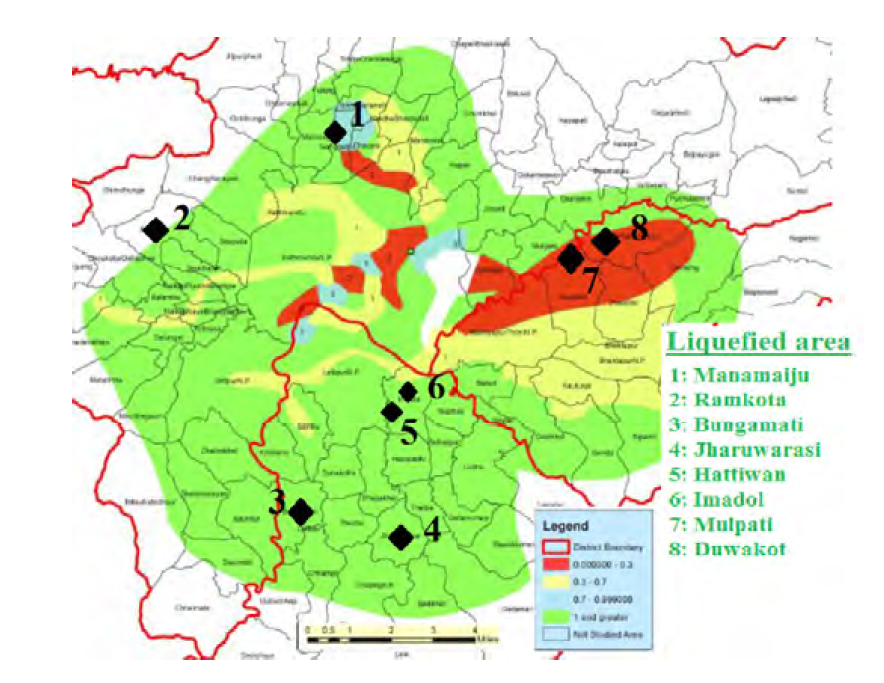
\includegraphics[width=0.75\linewidth,keepaspectratio]{images/main/dipendra.png}
\caption{Subedi et al. (2013), Liquefaction Susceptibility Map}
\end{figure}

Gautam et. Al(2015)\cite{r18} computed FS for various localities of Kathmandu Valley using borehole log and tallied those computed values of the sites where liquefaction actually occured during the 2015 gorkha earthquake.

\begin{figure}[!hbt]
\centering
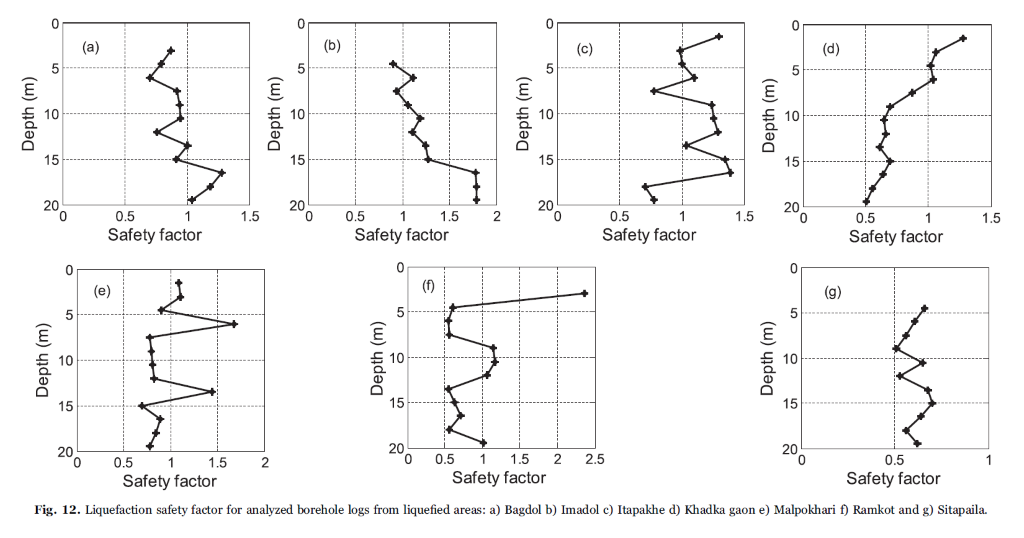
\includegraphics[width=0.75\linewidth,keepaspectratio]{images/main/bastola_acharya.png}
\caption{Liquefaction safety factor for for different borehole logs, D.Gautam et al.(2015)}
\end{figure}

Bastola and Acharya(2016)\cite{r31} prepared another using quantitative methods of  liquefaction susceptibility map preparation. Liquefaction Potential Index(LPI) was calculated for various borehole data and the area most prone to liquefaction was highlighted in the map. 

\subsection{Methods for liquefaction calculation}
There are qualitative and quantitative methods and deterministic and probabilistic approaches to assess the liquefaction potential. In this research, the stress-based approach suggested by Idriss and Boulanger\cite{idris_and_bolinger} has been adopted to perform an analysis of the factor of safety (FS) with respect to liquefaction on each layer and Iwasaki et al. \cite{r26} method has been used to estimate the liquefaction potential index(LPI) of the sites.
The stress-based approach for evaluating the potential 1-or liquefaction triggering, initiated by Seed and Idriss \cite{idris_seed}, has been used widely for the last 45 years. The basic framework, as adopted by numerous researchers, compares the earthquake-induced cyclic stress ratios (CSR) with the cyclic resistance ratios (CRR) of the soil. This method uses the Standard Penetration Test (SPT) blow count data and geotechnical properties of the soil layers to predict the earthquake potential.
\subsection{Stress based approach}
Stress based approach suggested by Idriss and Boulanger \cite{idris_and_bolinger} to find Factor of Safety. In this method, the stress (loading) that results in liquefaction is defined as the cyclic stress ratio (CSR), and the property of the soils to resist liquefaction is termed as the cyclic resistance ratio (CRR). The FS with respect to liquefaction can be calculated using:
\begin{equation}
FS = \frac{CRR}{CSR}
\end{equation}

Here, $CRR = CRR_{7.5}*M.S.F*K_\alpha $

Where, $CRR_{7.5}$ is the cyclic resistance ratio calibrated for the earthquake of magnitude 7.5; MSF is the magnitude scaling factor that accounts for the effects of shaking duration and $K_\alpha$ is a factor for the presence of sustained static shear stresses, which may exist beneath foundations or within slopes.

MSF and $K_\sigma$ were calculated using \cite{idris_and_bolinger}: 
\begin{equation}
MSF = 6.9 e^{- \frac{M_w}{4}} - 0.058 \leq 1.8
\end{equation}

Where,

Mw is magnitude of earthquake.
\begin{equation}
K_\sigma = 1 - C_\sigma ln (\frac{\sigma_v'}{P}) \leq 1.1
\end{equation}

Where,
$\sigma_v'$ is Vertical effective stress
$P$ is atmostpheric pressure at location
$C_\sigma$ is given as,

\begin{equation}
C_\sigma = \frac{1}{18.9-2.55\sqrt{({N_1})_{60cs}}} \leq 0.3
\end{equation}

$({N_1})_{60cs}$ is the corrected SPT value.

The $CRR_{7.5}$ is calculated using \cite{idris_and_bolinger}
\begin{equation}
CRR_{7.5} = exp(\frac{({N_1})_{60cs}}{14.1} + (\frac{({N_1})_{60cs}}{126})^2 + (\frac{({N_1})_{60cs}}{23.6})^3 + (\frac{({N_1})_{60cs}}{25.4})^4) - 2.8
\end{equation}

This provides cyclic resistance ratio for liquefaction of soil during earthquake. Here $({N_1})_{60cs}$ is corrected for fineness content in soil.

\begin{gather}
({N_1})_{60cs} = ({N_1})_{60} + \Delta({N_1})_{60} \\
\Delta({N_1})_{60} = exp(1.63 + \frac{9.7}{FC+0.01} + (\frac{15.7}{FC+0.01})^2 ) \\
\end{gather}

Here, FC is fines content in soils.

Cyclic stress ratio can be found using equation,

\begin{equation}
CSR = 0.65 \frac{\sigma_v}{\sigma_v'} \frac{a_{max}}{g} r_d
\end{equation}

Where,
$a_{max}$ is peak horizontal acceleration at surface.
$g$ is acceleration due to gravity.
$\sigma_v’$ is effective overburden stress.
$\sigma_v$ is total overburden stress.
Shear reduction factor rd is given by;

\begin{equation}
r_d = exp[ -1.012 - 1.126 (\frac{z}{11.73} + 5.133) + M_w( 0.106 + 0.118 \sin ( \frac{z}{11.28} +5.142 ) ) ]
\end{equation}

Here, z is the soil depth in m.

\subsection{Liquefaction potential index}
We consider 20 m depth for analysis of liquefaction potential of soil. Higher weightage is given to uppermost layers of soil as top layers are more responsible for liquefaction. We use Iwasaki et al. method to obtain liquefaction potential index by integrating safety factors on upper 20 m soil column as follows.

\begin{equation}
LPI = \int_{0}^{20} F(z).W(z).dz
\end{equation}

Where,
LPI is liquefaction potential index 

F(z) is function of safety factor (FS) given by,

\begin{math}
F(z) = \begin{cases}
	0, & \text{for} FS > 1.2 \\
	2*10^6 e^{-18.427 FS}, & \text{for} 1.2 \geq FS > 0.95 \\
	1-FS, & \text{for FS} \leq 0.95 \\
	\end{cases}
\end{math}

W(z) is  depth dependent factor which can be expressed as 

\begin{equation}
W(z) = 10 - 0.5 z
\end{equation}

But instead of above given integral we estimate the integral using summation given as,
\begin{equation}
LPI = \sum_ F(z).W(z). \delta z
\end{equation}